\indent \textbf{Greedy Forwarding}はGPSRの基本的な
ルーティングプロトコルである. 図\ref{fig:greedy}に示すように, 
送信ノードSは, 宛先ノードDの位置情報をもとに
自身の電波伝搬範囲内のノードから, Dに最も近いノードを
ネクストホップとして選択する. 前提として, 送信ノードSは宛先ノードDの
位置情報を事前に把握しているものとする. 点線で書かれた円は全ノードの
受信感度が等しい場合の送信ノードSの電波伝搬範囲を, 
破線は宛先ノードとの距離を表している.

\begin{figure}
  \centering
  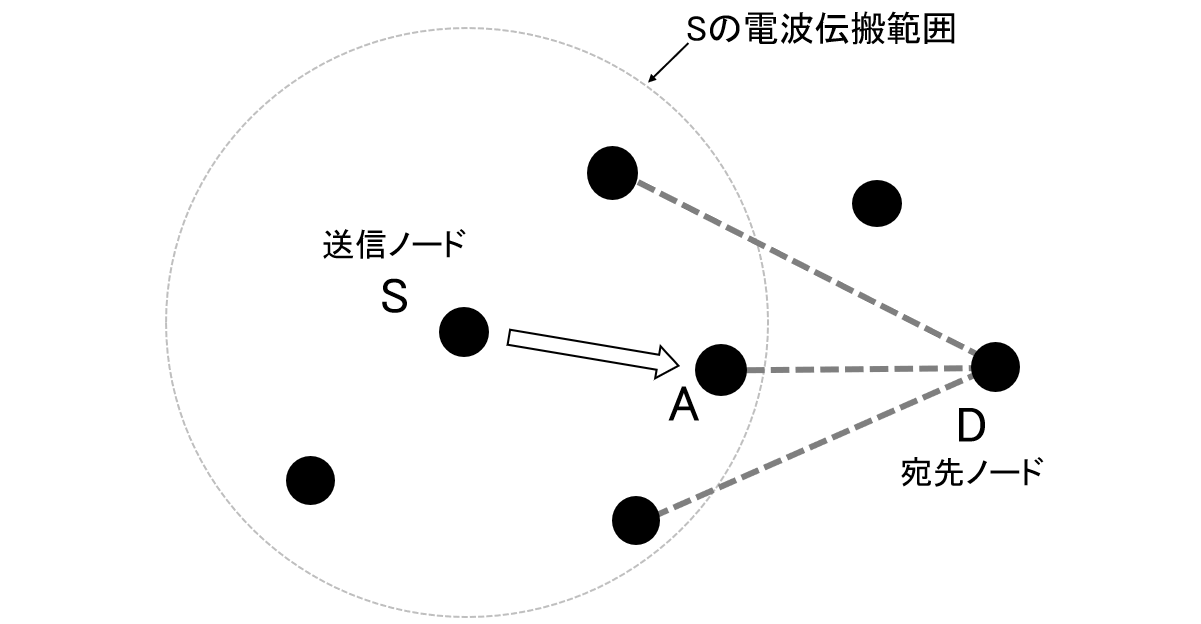
\includegraphics[scale=0.55]{figures/greedy.png}
  \caption{Greedy Forwarding}
  \label{fig:greedy}
\end{figure}

Greedy Forwardingでは局所最大問題と呼ばれる問題が生じてしまうことがある. 
\textbf{局所最大問題}とは, 図\ref{fig:local}に示すように, 送信ノードSの電波伝搬範囲内に
宛先ノードDが存在しない, かつ, 送信ノードSが自身の
電波伝搬範囲内で宛先ノードDに最も近い場合, 選択できる
ネクストホップが存在しなくなるという問題である.

\begin{figure}
  \centering
  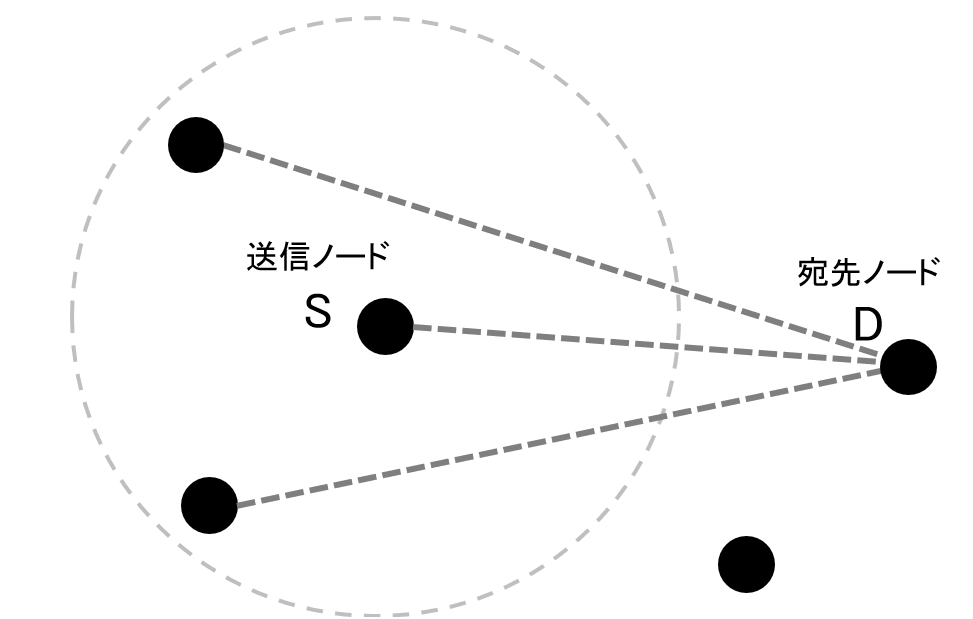
\includegraphics[scale=0.55]{figures/local.png}
  \caption{局所最大問題}
  \label{fig:local}
\end{figure}
